\newcommand{\institut}{}
\newcommand{\fachgebiet}{Regelungstechnik}
\newcommand{\veranstaltung}{Praktikum Grundlagen der Regelungstechnik}
\newcommand{\pdfautor}{Dirk Barbendererde (321 836), Boris Henckell (325 779)}
\newcommand{\autor}{Dirk Barbendererde (321 836)\\ Boris Henckell (325 779)}
\newcommand{\pdftitle}{Praktikum Regelungstechnik  Versuch 1b}
\newcommand{\prototitle}{Praktikum Regelungstechnik \\ Versuch 1b}
\newcommand{\aufgabe}{}

\newcommand{\gruppe}{Gruppe: G1 Di 12-14}
\newcommand{\betreuer}{Betreuer: Christian Schmuck}



\input{../../packages/tu_header_8}


% \lstlistoflistings
\definecolor{darkgray}{rgb}{0.95,0.95,0.95}
\lstset{language=Scilab}
\lstset{inputencoding=utf8}
%\lstset{extendedchars=true} % Umlaute an der richtigen stelle und nicht am Anfang ausgeben
\lstset{backgroundcolor=\color{darkgray}}
\lstset{numbers=left, numberstyle=\tiny, stepnumber=1, numbersep=7pt, breaklines=true}
\lstset{keywordstyle=\color{red}\bfseries\emph}
\lstset{
breaklines,
numbers=left,
frame=single,
xleftmargin=-2cm,
xrightmargin=-1.5cm
}
% enables UTF-8 in source code: (dirty, dirty hack)
\lstset{literate=
    %Deutsch
    {ä}{{\"a}}1 {ö}{{\"o}}1 {ü}{{\"u}}1 {Ä}{{\"A}}1 {Ö}
    {{\"O}}1 {Ü}{{\"U}}1 {ß}{\ss}1
    %Türkisch
    {â}{{\^{a}}}1 {Â}{{\^{A}}}1 {ç}{{\c{c}}}1 {Ç}{{\c{C}}}1 {ğ}{{\u{g}}}1 {Ğ}{{\u{G}}}1 {ı}{{\i}}1 {İ}{{\.{I}}}1 {ö}{{\"o}}1 {Ö}{{\"O}}1 {ş}{{\c{s}}}1
    {Ş}{{\c{S}}}1 {ü}{{\"u}}1 {Ü}{{\"U}}1
    %Polish
    {ą}{{\k{a}}}1 {ć}{{\'c}}1 {ę}{{\k{e}}}1 {ł}{{\l{}}}1 {ń}{{\'n}}1 {ó}{{\'o}}1 {ś}{{\'s}}1 {ż}{{\.z}}1 {ź}{{\'z}}1 {Ą}{{\k{A}}}1 {Ć}{{\'C}}1
    {Ę}{{\k{E}}}1 {Ł}{{\L{}}}1 {Ń}{{\'N}}1 {Ó}{{\'O}}1 {Ś}{{\'S}}1 {Ż}{{\.Z}}1 {Ź}{{\'Z}}1
    %Spanish
    {á}{{\'a}}1 {é}{{\'e}}1 {í}{{\'i}}1 {ó}{{\'o}}1 {ú}{{\'u}}1 {ñ}{{\~n}}1
}

%     \lstinputlisting{./praktikum6.sce}



%---------------------------------------------------------------------
%---------------------------------------------------------------------
%---------------------------------------------------------------------

\section{Vorbereitungsaufgaben}
\begin{quote}
	\subsection{Übertragungsfunktion}
    \hspace{-2em}
    Aufgabe:
    \hspace{-2em}Ermittlen Sie die Übertragungsfunktion $G_\omega^{'} (s) = \frac{\Omega(s)}{R_i (s)}$ der nun relevanten
    Regelstrecke, die den unterlagerten Stromregelkreis aus Versuchsteil 1a enthält.\\
	\begin{quote}
	   Zuerst errechnen wir die Zweite Regelstrecke $G_2$:\\
	   Der Zustandsvektor $x(t)$ besteht aus der Winkelgeschwindigkeit $\omega$.
        \begin{equation*}
            \begin{split}
                x(t) = 
                    \begin {pmatrix}
                        \omega(t)\\
                    \end{pmatrix}
            \end{split}
        \end{equation*}
        
        Die Stellgröße $u(t)$ besteht aus dem Ankerstrom $i_A(t)$.
        \begin{equation*}
            \begin{split}
                u(t) = i_A (t)
            \end{split}
        \end{equation*}
        
        Als Ausgangsgröße $y(t)$ wird die Winkelgeschwindigkeit $\omega$ genommen.
        \begin{equation*}
            \begin{split}
                y(t) = \omega(t)
            \end{split}
        \end{equation*}
        
        Daraus ergibt sich folgendes Zustandesmodell:
        \begin{equation*}
            \begin{split}
                   \dot{x} &=
                   \begin{pmatrix}
                        \dot{\omega}(t)\\
                   \end{pmatrix}\\ &=
                   \begin{pmatrix}
                        -\frac{c_\mu}{\frac{1}{2}M_s r^2_s + J_m}\\
                   \end{pmatrix} x(t) +
                   \begin{pmatrix}
                       \frac{k_m}{\frac{1}{2}M_sr^2_s + J_m}\\
                   \end{pmatrix} u(t) +
                   \begin{pmatrix}
                       \frac{-1}{\frac{1}{2}M_sr^2_s + J_m}\\
                   \end{pmatrix} m_L(t)\\
                   y(t) &= 
                   \begin{pmatrix}
                        1\\
                   \end{pmatrix} x(t) + 0u(t)
            \end{split}
        \end{equation*}
        
        Daraus folgt folgende Übertragungsfunktion $G_2$:
        \begin{equation*}
        	\begin{split}
        		G_2 (s) = \frac{2351,6287}{0,0178492 + s}
        	\end{split}
        \end{equation*}
        
        Nun können wir $G_\omega^{'}$ berechnen:
	
		\begin{equation*}
        	\begin{split}
        		G_\omega^{'} (s) &= T_1(s) G_2(s) = \frac{G_1 (s) K_1(s)}{1 + G_1 (s) K_1 (s)} G_2 (s)\\ \\
        		&= \frac{475559.23}{3.6095577 + 202.24332s + s^2}
        	\end{split}
        \end{equation*}
		
        
	\end{quote}
	
	\subsection{Regler}
    Aufgabe:\\
    Als Drehzahlregler soll ein PI-Glied\\
    \begin{equation*}
        \begin{split}
            K_\omega (s) = k_\omega \frac{s-s_{0,\omega}}{s}, \hspace{2em} k_\omega, s_{0,\omega} \in \mathbb{R}
        \end{split}
    \end{equation*}
    verwendet werden.
	\begin{quote}
		
		\subsubsection{Begründen}
        Aufgabe:\\
        Begründen Sie, warum diese Reglerstruktur sinnvoll ist.\\
		\begin{quote}
			
		\end{quote}
		
		\subsubsection{Bode-Diagramm}
        Aufgabe:\\
        Der Reglerentwurf soll nach dem Frequenzkennlinienverfahren durchgeführt werden. Zeichnen Sie dafür zunächst
        das Bode-Diagramm von $G_\omega^{'}$.\\   
        \begin{quote}
            \begin{figure}[H]
            \centering
                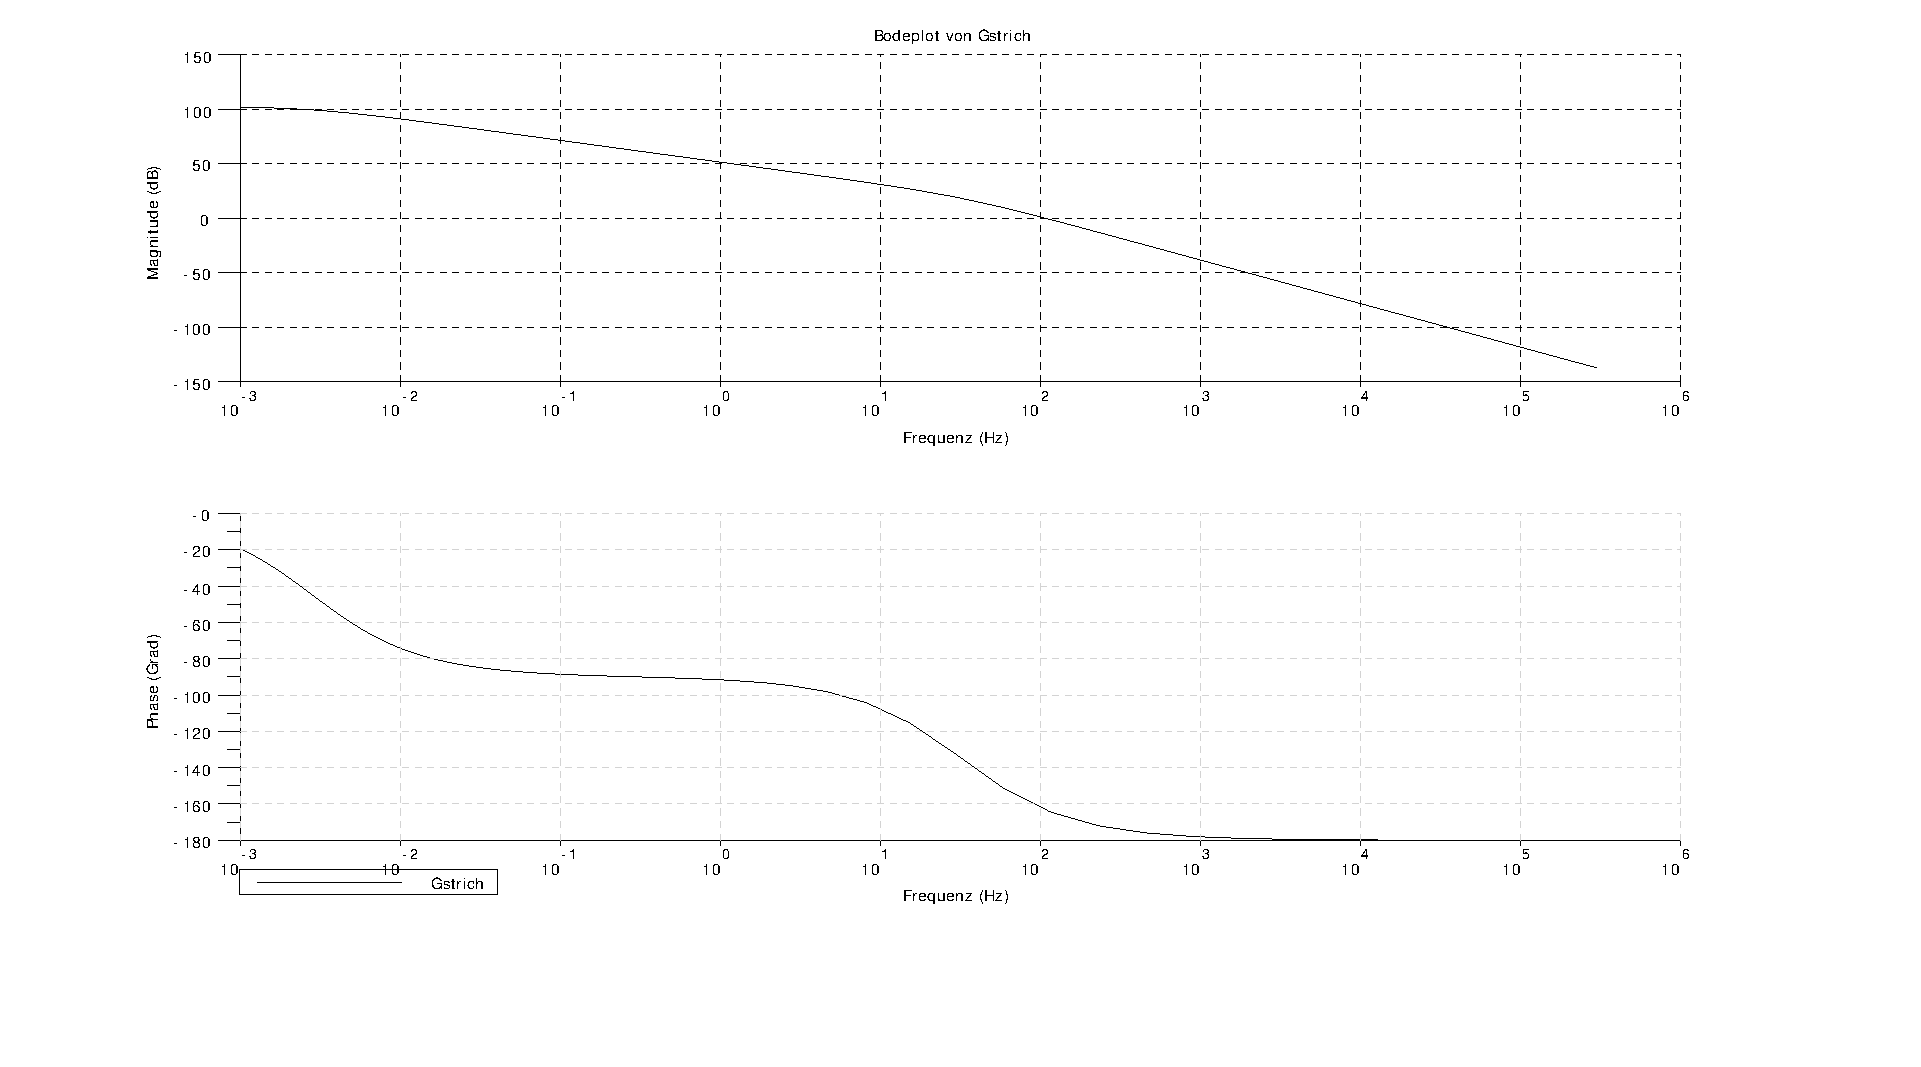
\includegraphics[scale=0.5, trim = 0cm 0cm 0cm 0cm, clip]{./Bilder/BodevonGstrich}
                    \caption{caption}
                    \label{fig:BodevonGstrich}
            \end{figure}
       
        \end{quote}

        \subsubsection{Reglerentwurf}
        Aufgabe:\\        
        Wählen Sie zunächst das aus der Vorlesung bekannte Entwurfsvorgehen, indem Sie mit der Nullstelle $s_{0,\omega}$
        des Reglers die langsamste Polstelle der Strecke kürzen. Bestimmen Sie dann mit Hilfe von Simulationen die
        Verstärkung $k_\omega$ so, dass der geschlossene Regelkreis eine Ausregelzeit von etwa $0.6$ Sekunden aufweist
        und das Ü̈berschwingen einen Wert von $20\%$ nicht übersteigt. Rufen Sie sich in Erinnerung, wie die
        Kenngrößen ``Überschwingweite'' , ``Ausregelzeit'' , ``Phasenreserve'' und ``Durchtrittsfrequenz''
        miteinander in Beziehung stehen!
        \begin{quote} 
            ``Überschwingweite'': Bei der Überschwingweite handelt es sich um die maximale Abweichung der Reglegröße vom
            Sollwert, $\Delta y = max(y) - y_{soll}$, nach dem die Relgröße die Sollgröße überschritten hat.       
            \cite{Ueberschwingweite}
            
            
            
            
            
            
            \vspace{2em}
            Phasenreserve und Überschwingweite hängen folgendermaßen zusammen:\\
            \begin{equation}
                \begin{split}
                \varphi_R [^\circ] + e_{max} [\%] \approx 70
                \end{split}
            \end{equation}
            
            \vspace{1em}
            Auch Amplitudenreserve und Anstiegszeit hängen voneinander ab. Je kürzer die Anstiegszeit ist desto
            höher ist die maximale Überschwingweite und desto geringer ist auch die Amplitudenreserve. In
            der Praxis wird oft auch der Zusammenhang von Durchtrittsfrequenz und Anstiegszeit
            verwendet:
            \begin{equation}
            \begin{split}
                \omega_D = \frac{1}{T_{a,50}} \p (1,5- \frac{e_{max} [\%]}{250})
            \end{split}
            \end{equation}
            \cite{krachler}
        \end{quote}
        
        \subsubsection{Erstellen der Führungsübertragungsfunktion}
        Aufgabe:\\
        Bei Sprüngen der Führungsgröße $r_\omega$ von $0$ auf Werte bis zu $180 \frac{rad}{s}$ soll die
        Stellgrößenbeschränkung von $−5V < u < 5V$ nicht verletzt werden. Überprüfen Sie simulativ, ob Ihr Regler
        diese Forderung erfüllt. Falls nicht, korrigieren Sie ihre Reglerparameter, sodass die Forderung erfüllt wird.
        Wie lautet die Übertragungsfunktion $\overline{T}_\omega$ des bis hierhin entworfenen geschlossenen
        Regelkreises?
        \begin{quote}
            \begin{equation*}
            	\begin{split}
            		\overline{T}_\omega &= \frac{G_\omega^{'} K_\omega}{1 + G_\omega^{'} K_\omega}\\
            		&= \frac{1531.9576s +  171663.42s^2 +  4809358.2s^3 +  23777.961s^4}{1531.9576s +  171676.45s^2 + 
            		4810818.3s^3 +  64687.541s^4 +  404.48664s^5 +  1s^6}
            	\end{split}
            \end{equation*}
        \end{quote}
        
        \subsubsection{Erstellen der Störübertragungsfunktion}
        Aufgabe:\\
        Berechnen Sie die Störübertragungsfunktion $\overline{G}_{m\omega} (s) = \frac{\Omega(s)}{M_L (s)}$ vom
        Lastmoment $m_L$ auf die Winkelgeschwindigkeit $\omega$. Simulieren Sie die Störsprungantwort. Warum ist das
        Störverhalten des entworfenen Regelkreises nicht brauchbar? Was fällt Ihnen auf, wenn Sie die Pole von
        $\overline{T}_\omega$ und $\overline{G}_\omega$ vergleichen?
		\begin{quote}
			\begin{equation*}
            	\begin{split}
            		\overline{G}_{m\omega} (s) = \frac{\Omega(s)}{M_L (s)} = \frac{1}{1+ G_\omega^{'} T_\omega}
            	\end{split}
            \end{equation*}
		\end{quote}
		
		\subsubsection{Korrektur der Führungs- und Störübertragungsfunktion}
		Aufgabe:\\
	    Überlegen Sie mit Hilfe der Wurzelortskurve, wie die Nullstelle $s_{0,ω}$ des Reglers verschoben werden muss, um
	    das Störverhalten zu verbessern. Wählen Sie $s_{0,ω}$ und $k_\omega$ neu, sodass alle vorher genannten
	    Forderungen an das Führungsverhalten weiterhin erfüllt werden. Wie lauten die neue
	    Führungsübertragungsfunktion $T_\omega$ und die neue Störübertragungsfunktion $G_{m\omega}$ und deren Pole?
		\begin{quote}
			
		\end{quote}
		
	\end{quote}
	
	\subsection{Anti-Windup-Schaltung in Scicos erstellen}
	Aufgabe:\\
    Erweitern Sie Ihre Reglerstruktur in Scicos um eine Anti-Windup-Schaltung nach Abbildung 11. Beziehen Sie sowohl
    den äußeren als auch den inneren Regler in die Schaltung ein. Realisieren Sie dafür den inneren und äußeren
    PI-Regler in einer Parallelform mit P- und I-Anteil.
	\begin{quote}
		
		
	\end{quote}
	
\end{quote}

%--------------------------------------------------------------------
%--------------------------------------------------------------------

\section{Versuch}
\begin{quote}
    
\end{quote}

%--------------------------------------------------------------------
%--------------------------------------------------------------------

\section{Ergebnisse}
\begin{quote}
    
\end{quote}

%--------------------------------------------------------------------
%--------------------------------------------------------------------



% \begin{quote}
%     \lstinputlisting[
%         caption={Scilab-script},
%         label=lst:scilab]
%         {./Scilab/Motor.sce}
%         
% \end{quote}

%--------------------------------------------------------------------
%--------------------------------------------------------------------
\begin{thebibliography}{999}
\bibitem {Ueberschwingweite} Prof. Dr.-Ing. Raisch, Jörg; Dipl.-Ing. Hess, Anne-Katrin; Dipl.-Ing. Seel, Thomas:
Grundlagen der Regelungstechnik - 4.Praktikum, S.5

\bibitem{krachler}Christian Krachler:
Reglersynthese nach dem Frequenzkennlinienverfahren, S16, S22

%Name, Vorname.; evtl. Name2, Vorname2.: Titel des Dokumentes
%oder Buches, Zeitschrift/Verlag/URL (Auflage, Erscheinungsort, -jahr), ggf. Seitenzahlen
%\bibitem [Wiki10] {DigitaleMesskette2} \url{www.wikipedia.org}, Zugriff 22.03.2010
\end{thebibliography}


\end{document}
